% Created by tikzDevice version 0.12.6 on 2024-07-02 15:00:12
% !TEX encoding = UTF-8 Unicode
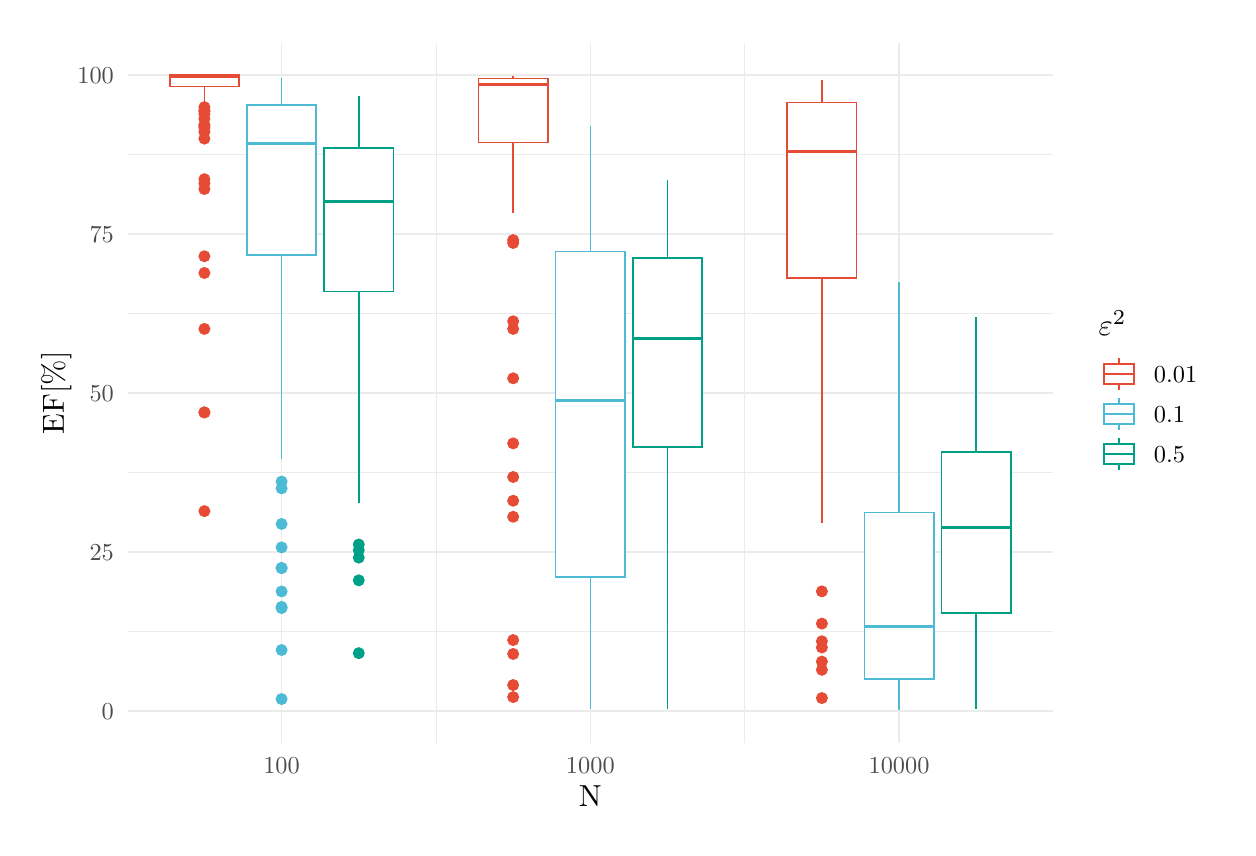
\begin{tikzpicture}[x=1pt,y=1pt]
\definecolor{fillColor}{RGB}{255,255,255}
\path[use as bounding box,fill=fillColor,fill opacity=0.00] (0,0) rectangle (433.62,289.08);
\begin{scope}
\path[clip] ( 36.11, 30.69) rectangle (370.53,283.58);
\definecolor{drawColor}{gray}{0.92}

\path[draw=drawColor,line width= 0.3pt,line join=round] ( 36.11, 70.92) --
	(370.53, 70.92);

\path[draw=drawColor,line width= 0.3pt,line join=round] ( 36.11,128.39) --
	(370.53,128.39);

\path[draw=drawColor,line width= 0.3pt,line join=round] ( 36.11,185.87) --
	(370.53,185.87);

\path[draw=drawColor,line width= 0.3pt,line join=round] ( 36.11,243.35) --
	(370.53,243.35);

\path[draw=drawColor,line width= 0.3pt,line join=round] (147.54, 30.69) --
	(147.54,283.58);

\path[draw=drawColor,line width= 0.3pt,line join=round] (259.10, 30.69) --
	(259.10,283.58);

\path[draw=drawColor,line width= 0.6pt,line join=round] ( 36.11, 42.18) --
	(370.53, 42.18);

\path[draw=drawColor,line width= 0.6pt,line join=round] ( 36.11, 99.66) --
	(370.53, 99.66);

\path[draw=drawColor,line width= 0.6pt,line join=round] ( 36.11,157.13) --
	(370.53,157.13);

\path[draw=drawColor,line width= 0.6pt,line join=round] ( 36.11,214.61) --
	(370.53,214.61);

\path[draw=drawColor,line width= 0.6pt,line join=round] ( 36.11,272.08) --
	(370.53,272.08);

\path[draw=drawColor,line width= 0.6pt,line join=round] ( 91.75, 30.69) --
	( 91.75,283.58);

\path[draw=drawColor,line width= 0.6pt,line join=round] (203.32, 30.69) --
	(203.32,283.58);

\path[draw=drawColor,line width= 0.6pt,line join=round] (314.88, 30.69) --
	(314.88,283.58);
\definecolor{drawColor}{RGB}{230,75,53}
\definecolor{fillColor}{RGB}{230,75,53}

\path[draw=drawColor,line width= 0.4pt,line join=round,line cap=round,fill=fillColor] ( 63.86,251.38) circle (  1.96);

\path[draw=drawColor,line width= 0.4pt,line join=round,line cap=round,fill=fillColor] ( 63.86,248.98) circle (  1.96);

\path[draw=drawColor,line width= 0.4pt,line join=round,line cap=round,fill=fillColor] ( 63.86,180.22) circle (  1.96);

\path[draw=drawColor,line width= 0.4pt,line join=round,line cap=round,fill=fillColor] ( 63.86,206.48) circle (  1.96);

\path[draw=drawColor,line width= 0.4pt,line join=round,line cap=round,fill=fillColor] ( 63.86,254.00) circle (  1.96);

\path[draw=drawColor,line width= 0.4pt,line join=round,line cap=round,fill=fillColor] ( 63.86,259.06) circle (  1.96);

\path[draw=drawColor,line width= 0.4pt,line join=round,line cap=round,fill=fillColor] ( 63.86,150.08) circle (  1.96);

\path[draw=drawColor,line width= 0.4pt,line join=round,line cap=round,fill=fillColor] ( 63.86,256.14) circle (  1.96);

\path[draw=drawColor,line width= 0.4pt,line join=round,line cap=round,fill=fillColor] ( 63.86,234.33) circle (  1.96);

\path[draw=drawColor,line width= 0.4pt,line join=round,line cap=round,fill=fillColor] ( 63.86,252.89) circle (  1.96);

\path[draw=drawColor,line width= 0.4pt,line join=round,line cap=round,fill=fillColor] ( 63.86,232.80) circle (  1.96);

\path[draw=drawColor,line width= 0.4pt,line join=round,line cap=round,fill=fillColor] ( 63.86,230.78) circle (  1.96);

\path[draw=drawColor,line width= 0.4pt,line join=round,line cap=round,fill=fillColor] ( 63.86,260.36) circle (  1.96);

\path[draw=drawColor,line width= 0.4pt,line join=round,line cap=round,fill=fillColor] ( 63.86,253.55) circle (  1.96);

\path[draw=drawColor,line width= 0.4pt,line join=round,line cap=round,fill=fillColor] ( 63.86,258.87) circle (  1.96);

\path[draw=drawColor,line width= 0.4pt,line join=round,line cap=round,fill=fillColor] ( 63.86,114.39) circle (  1.96);

\path[draw=drawColor,line width= 0.4pt,line join=round,line cap=round,fill=fillColor] ( 63.86,200.43) circle (  1.96);

\path[draw=drawColor,line width= 0.4pt,line join=round,line cap=round,fill=fillColor] ( 63.86,257.88) circle (  1.96);

\path[draw=drawColor,line width= 0.4pt,line join=round,line cap=round,fill=fillColor] ( 63.86,150.02) circle (  1.96);

\path[draw=drawColor,line width= 0.6pt,line join=round] ( 63.86,271.93) -- ( 63.86,272.07);

\path[draw=drawColor,line width= 0.6pt,line join=round] ( 63.86,267.84) -- ( 63.86,262.13);
\definecolor{fillColor}{RGB}{255,255,255}

\path[draw=drawColor,line width= 0.6pt,fill=fillColor] ( 51.31,271.93) --
	( 51.31,267.84) --
	( 76.41,267.84) --
	( 76.41,271.93) --
	( 51.31,271.93) --
	cycle;

\path[draw=drawColor,line width= 1.1pt] ( 51.31,271.62) -- ( 76.41,271.62);
\definecolor{drawColor}{RGB}{77,187,213}
\definecolor{fillColor}{RGB}{77,187,213}

\path[draw=drawColor,line width= 0.4pt,line join=round,line cap=round,fill=fillColor] ( 91.75,109.75) circle (  1.96);

\path[draw=drawColor,line width= 0.4pt,line join=round,line cap=round,fill=fillColor] ( 91.75, 79.34) circle (  1.96);

\path[draw=drawColor,line width= 0.4pt,line join=round,line cap=round,fill=fillColor] ( 91.75,101.28) circle (  1.96);

\path[draw=drawColor,line width= 0.4pt,line join=round,line cap=round,fill=fillColor] ( 91.75, 46.48) circle (  1.96);

\path[draw=drawColor,line width= 0.4pt,line join=round,line cap=round,fill=fillColor] ( 91.75, 64.19) circle (  1.96);

\path[draw=drawColor,line width= 0.4pt,line join=round,line cap=round,fill=fillColor] ( 91.75, 93.88) circle (  1.96);

\path[draw=drawColor,line width= 0.4pt,line join=round,line cap=round,fill=fillColor] ( 91.75, 93.76) circle (  1.96);

\path[draw=drawColor,line width= 0.4pt,line join=round,line cap=round,fill=fillColor] ( 91.75,122.61) circle (  1.96);

\path[draw=drawColor,line width= 0.4pt,line join=round,line cap=round,fill=fillColor] ( 91.75, 85.36) circle (  1.96);

\path[draw=drawColor,line width= 0.4pt,line join=round,line cap=round,fill=fillColor] ( 91.75, 79.78) circle (  1.96);

\path[draw=drawColor,line width= 0.4pt,line join=round,line cap=round,fill=fillColor] ( 91.75,125.06) circle (  1.96);

\path[draw=drawColor,line width= 0.6pt,line join=round] ( 91.75,261.10) -- ( 91.75,270.84);

\path[draw=drawColor,line width= 0.6pt,line join=round] ( 91.75,206.87) -- ( 91.75,133.20);
\definecolor{fillColor}{RGB}{255,255,255}

\path[draw=drawColor,line width= 0.6pt,fill=fillColor] ( 79.20,261.10) --
	( 79.20,206.87) --
	(104.30,206.87) --
	(104.30,261.10) --
	( 79.20,261.10) --
	cycle;

\path[draw=drawColor,line width= 1.1pt] ( 79.20,247.32) -- (104.30,247.32);
\definecolor{drawColor}{RGB}{0,160,135}
\definecolor{fillColor}{RGB}{0,160,135}

\path[draw=drawColor,line width= 0.4pt,line join=round,line cap=round,fill=fillColor] (119.64,102.33) circle (  1.96);

\path[draw=drawColor,line width= 0.4pt,line join=round,line cap=round,fill=fillColor] (119.64,100.27) circle (  1.96);

\path[draw=drawColor,line width= 0.4pt,line join=round,line cap=round,fill=fillColor] (119.64, 97.58) circle (  1.96);

\path[draw=drawColor,line width= 0.4pt,line join=round,line cap=round,fill=fillColor] (119.64, 89.37) circle (  1.96);

\path[draw=drawColor,line width= 0.4pt,line join=round,line cap=round,fill=fillColor] (119.64, 63.06) circle (  1.96);

\path[draw=drawColor,line width= 0.6pt,line join=round] (119.64,245.64) -- (119.64,264.45);

\path[draw=drawColor,line width= 0.6pt,line join=round] (119.64,193.75) -- (119.64,117.25);
\definecolor{fillColor}{RGB}{255,255,255}

\path[draw=drawColor,line width= 0.6pt,fill=fillColor] (107.09,245.64) --
	(107.09,193.75) --
	(132.20,193.75) --
	(132.20,245.64) --
	(107.09,245.64) --
	cycle;

\path[draw=drawColor,line width= 1.1pt] (107.09,226.34) -- (132.20,226.34);
\definecolor{drawColor}{RGB}{230,75,53}
\definecolor{fillColor}{RGB}{230,75,53}

\path[draw=drawColor,line width= 0.4pt,line join=round,line cap=round,fill=fillColor] (175.43,126.72) circle (  1.96);

\path[draw=drawColor,line width= 0.4pt,line join=round,line cap=round,fill=fillColor] (175.43, 62.77) circle (  1.96);

\path[draw=drawColor,line width= 0.4pt,line join=round,line cap=round,fill=fillColor] (175.43,211.28) circle (  1.96);

\path[draw=drawColor,line width= 0.4pt,line join=round,line cap=round,fill=fillColor] (175.43, 47.19) circle (  1.96);

\path[draw=drawColor,line width= 0.4pt,line join=round,line cap=round,fill=fillColor] (175.43,182.99) circle (  1.96);

\path[draw=drawColor,line width= 0.4pt,line join=round,line cap=round,fill=fillColor] (175.43,212.32) circle (  1.96);

\path[draw=drawColor,line width= 0.4pt,line join=round,line cap=round,fill=fillColor] (175.43, 51.54) circle (  1.96);

\path[draw=drawColor,line width= 0.4pt,line join=round,line cap=round,fill=fillColor] (175.43,138.87) circle (  1.96);

\path[draw=drawColor,line width= 0.4pt,line join=round,line cap=round,fill=fillColor] (175.43,180.21) circle (  1.96);

\path[draw=drawColor,line width= 0.4pt,line join=round,line cap=round,fill=fillColor] (175.43, 67.79) circle (  1.96);

\path[draw=drawColor,line width= 0.4pt,line join=round,line cap=round,fill=fillColor] (175.43,162.38) circle (  1.96);

\path[draw=drawColor,line width= 0.4pt,line join=round,line cap=round,fill=fillColor] (175.43,112.33) circle (  1.96);

\path[draw=drawColor,line width= 0.4pt,line join=round,line cap=round,fill=fillColor] (175.43,118.13) circle (  1.96);

\path[draw=drawColor,line width= 0.6pt,line join=round] (175.43,270.66) -- (175.43,271.72);

\path[draw=drawColor,line width= 0.6pt,line join=round] (175.43,247.63) -- (175.43,222.28);
\definecolor{fillColor}{RGB}{255,255,255}

\path[draw=drawColor,line width= 0.6pt,fill=fillColor] (162.88,270.66) --
	(162.88,247.63) --
	(187.98,247.63) --
	(187.98,270.66) --
	(162.88,270.66) --
	cycle;

\path[draw=drawColor,line width= 1.1pt] (162.88,268.45) -- (187.98,268.45);
\definecolor{drawColor}{RGB}{77,187,213}

\path[draw=drawColor,line width= 0.6pt,line join=round] (203.32,208.19) -- (203.32,253.54);

\path[draw=drawColor,line width= 0.6pt,line join=round] (203.32, 90.60) -- (203.32, 43.02);

\path[draw=drawColor,line width= 0.6pt,fill=fillColor] (190.77,208.19) --
	(190.77, 90.60) --
	(215.87, 90.60) --
	(215.87,208.19) --
	(190.77,208.19) --
	cycle;

\path[draw=drawColor,line width= 1.1pt] (190.77,154.31) -- (215.87,154.31);
\definecolor{drawColor}{RGB}{0,160,135}

\path[draw=drawColor,line width= 0.6pt,line join=round] (231.21,205.74) -- (231.21,233.88);

\path[draw=drawColor,line width= 0.6pt,line join=round] (231.21,137.67) -- (231.21, 42.94);

\path[draw=drawColor,line width= 0.6pt,fill=fillColor] (218.66,205.74) --
	(218.66,137.67) --
	(243.76,137.67) --
	(243.76,205.74) --
	(218.66,205.74) --
	cycle;

\path[draw=drawColor,line width= 1.1pt] (218.66,176.71) -- (243.76,176.71);
\definecolor{drawColor}{RGB}{230,75,53}
\definecolor{fillColor}{RGB}{230,75,53}

\path[draw=drawColor,line width= 0.4pt,line join=round,line cap=round,fill=fillColor] (286.99, 57.04) circle (  1.96);

\path[draw=drawColor,line width= 0.4pt,line join=round,line cap=round,fill=fillColor] (286.99, 65.12) circle (  1.96);

\path[draw=drawColor,line width= 0.4pt,line join=round,line cap=round,fill=fillColor] (286.99, 60.01) circle (  1.96);

\path[draw=drawColor,line width= 0.4pt,line join=round,line cap=round,fill=fillColor] (286.99, 85.39) circle (  1.96);

\path[draw=drawColor,line width= 0.4pt,line join=round,line cap=round,fill=fillColor] (286.99, 73.74) circle (  1.96);

\path[draw=drawColor,line width= 0.4pt,line join=round,line cap=round,fill=fillColor] (286.99, 46.83) circle (  1.96);

\path[draw=drawColor,line width= 0.4pt,line join=round,line cap=round,fill=fillColor] (286.99, 67.36) circle (  1.96);

\path[draw=drawColor,line width= 0.6pt,line join=round] (286.99,262.03) -- (286.99,270.08);

\path[draw=drawColor,line width= 0.6pt,line join=round] (286.99,198.53) -- (286.99,110.21);
\definecolor{fillColor}{RGB}{255,255,255}

\path[draw=drawColor,line width= 0.6pt,fill=fillColor] (274.44,262.03) --
	(274.44,198.53) --
	(299.54,198.53) --
	(299.54,262.03) --
	(274.44,262.03) --
	cycle;

\path[draw=drawColor,line width= 1.1pt] (274.44,244.33) -- (299.54,244.33);
\definecolor{drawColor}{RGB}{77,187,213}

\path[draw=drawColor,line width= 0.6pt,line join=round] (314.88,113.84) -- (314.88,197.09);

\path[draw=drawColor,line width= 0.6pt,line join=round] (314.88, 53.80) -- (314.88, 42.37);

\path[draw=drawColor,line width= 0.6pt,fill=fillColor] (302.33,113.84) --
	(302.33, 53.80) --
	(327.43, 53.80) --
	(327.43,113.84) --
	(302.33,113.84) --
	cycle;

\path[draw=drawColor,line width= 1.1pt] (302.33, 72.66) -- (327.43, 72.66);
\definecolor{drawColor}{RGB}{0,160,135}

\path[draw=drawColor,line width= 0.6pt,line join=round] (342.77,135.84) -- (342.77,184.37);

\path[draw=drawColor,line width= 0.6pt,line join=round] (342.77, 77.54) -- (342.77, 42.91);

\path[draw=drawColor,line width= 0.6pt,fill=fillColor] (330.22,135.84) --
	(330.22, 77.54) --
	(355.32, 77.54) --
	(355.32,135.84) --
	(330.22,135.84) --
	cycle;

\path[draw=drawColor,line width= 1.1pt] (330.22,108.44) -- (355.32,108.44);
\end{scope}
\begin{scope}
\path[clip] (  0.00,  0.00) rectangle (433.62,289.08);
\definecolor{drawColor}{gray}{0.30}

\node[text=drawColor,anchor=base east,inner sep=0pt, outer sep=0pt, scale=  0.88] at ( 31.16, 39.15) {0};

\node[text=drawColor,anchor=base east,inner sep=0pt, outer sep=0pt, scale=  0.88] at ( 31.16, 96.63) {25};

\node[text=drawColor,anchor=base east,inner sep=0pt, outer sep=0pt, scale=  0.88] at ( 31.16,154.10) {50};

\node[text=drawColor,anchor=base east,inner sep=0pt, outer sep=0pt, scale=  0.88] at ( 31.16,211.58) {75};

\node[text=drawColor,anchor=base east,inner sep=0pt, outer sep=0pt, scale=  0.88] at ( 31.16,269.05) {100};
\end{scope}
\begin{scope}
\path[clip] (  0.00,  0.00) rectangle (433.62,289.08);
\definecolor{drawColor}{gray}{0.30}

\node[text=drawColor,anchor=base,inner sep=0pt, outer sep=0pt, scale=  0.88] at ( 91.75, 19.68) {100};

\node[text=drawColor,anchor=base,inner sep=0pt, outer sep=0pt, scale=  0.88] at (203.32, 19.68) {1000};

\node[text=drawColor,anchor=base,inner sep=0pt, outer sep=0pt, scale=  0.88] at (314.88, 19.68) {10000};
\end{scope}
\begin{scope}
\path[clip] (  0.00,  0.00) rectangle (433.62,289.08);
\definecolor{drawColor}{RGB}{0,0,0}

\node[text=drawColor,anchor=base,inner sep=0pt, outer sep=0pt, scale=  1.10] at (203.32,  7.64) {N};
\end{scope}
\begin{scope}
\path[clip] (  0.00,  0.00) rectangle (433.62,289.08);
\definecolor{drawColor}{RGB}{0,0,0}

\node[text=drawColor,rotate= 90.00,anchor=base,inner sep=0pt, outer sep=0pt, scale=  1.10] at ( 13.08,157.13) {EF[\%]};
\end{scope}
\begin{scope}
\path[clip] (  0.00,  0.00) rectangle (433.62,289.08);
\definecolor{drawColor}{RGB}{0,0,0}

\node[text=drawColor,anchor=base west,inner sep=0pt, outer sep=0pt, scale=  1.10] at (387.03,177.78) {$\varepsilon^2$};
\end{scope}
\begin{scope}
\path[clip] (  0.00,  0.00) rectangle (433.62,289.08);
\definecolor{drawColor}{RGB}{230,75,53}

\path[draw=drawColor,line width= 0.6pt] (394.25,158.20) --
	(394.25,160.37);

\path[draw=drawColor,line width= 0.6pt] (394.25,167.59) --
	(394.25,169.76);
\definecolor{fillColor}{RGB}{255,255,255}

\path[draw=drawColor,line width= 0.6pt,fill=fillColor] (388.83,160.37) rectangle (399.67,167.59);

\path[draw=drawColor,line width= 0.6pt] (388.83,163.98) --
	(399.67,163.98);
\end{scope}
\begin{scope}
\path[clip] (  0.00,  0.00) rectangle (433.62,289.08);
\definecolor{drawColor}{RGB}{77,187,213}

\path[draw=drawColor,line width= 0.6pt] (394.25,143.74) --
	(394.25,145.91);

\path[draw=drawColor,line width= 0.6pt] (394.25,153.14) --
	(394.25,155.31);
\definecolor{fillColor}{RGB}{255,255,255}

\path[draw=drawColor,line width= 0.6pt,fill=fillColor] (388.83,145.91) rectangle (399.67,153.14);

\path[draw=drawColor,line width= 0.6pt] (388.83,149.53) --
	(399.67,149.53);
\end{scope}
\begin{scope}
\path[clip] (  0.00,  0.00) rectangle (433.62,289.08);
\definecolor{drawColor}{RGB}{0,160,135}

\path[draw=drawColor,line width= 0.6pt] (394.25,129.29) --
	(394.25,131.46);

\path[draw=drawColor,line width= 0.6pt] (394.25,138.69) --
	(394.25,140.85);
\definecolor{fillColor}{RGB}{255,255,255}

\path[draw=drawColor,line width= 0.6pt,fill=fillColor] (388.83,131.46) rectangle (399.67,138.69);

\path[draw=drawColor,line width= 0.6pt] (388.83,135.07) --
	(399.67,135.07);
\end{scope}
\begin{scope}
\path[clip] (  0.00,  0.00) rectangle (433.62,289.08);
\definecolor{drawColor}{RGB}{0,0,0}

\node[text=drawColor,anchor=base west,inner sep=0pt, outer sep=0pt, scale=  0.88] at (406.98,160.95) {0.01};
\end{scope}
\begin{scope}
\path[clip] (  0.00,  0.00) rectangle (433.62,289.08);
\definecolor{drawColor}{RGB}{0,0,0}

\node[text=drawColor,anchor=base west,inner sep=0pt, outer sep=0pt, scale=  0.88] at (406.98,146.50) {0.1};
\end{scope}
\begin{scope}
\path[clip] (  0.00,  0.00) rectangle (433.62,289.08);
\definecolor{drawColor}{RGB}{0,0,0}

\node[text=drawColor,anchor=base west,inner sep=0pt, outer sep=0pt, scale=  0.88] at (406.98,132.04) {0.5};
\end{scope}
\end{tikzpicture}
